\chapter{}

\section{App}
The demo app is inspired by the tutorial \href{https://developer.android.com/courses/android-basics-compose/unit-1}{Unit 1: Your first Android App} on the Android Studio website. It features a background image and a content part devised sections using the \textsl{Column} and\textsl{Box} environment for composables. We present a name in coloured letters with a circular profile picture beneath. Further down we see a small bio section and a contact email address.
In Fig. \ref{fig:app_screen} we see screenshots of the app screen in both the built-in previewer and the emulator of Android Studio.


\begin{figure}
	\centering
	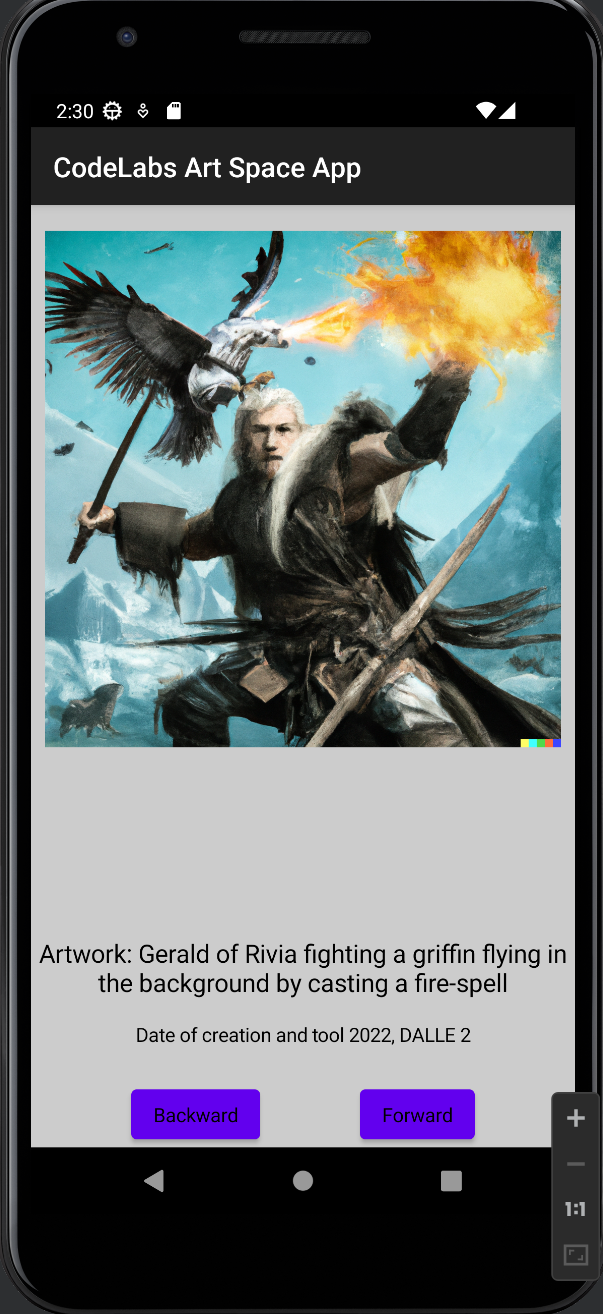
\includegraphics[width=.3\linewidth]{figures/app_screenshot_1.png}
	\caption{Screenshot of app screen in preview windows of Android Studio}
	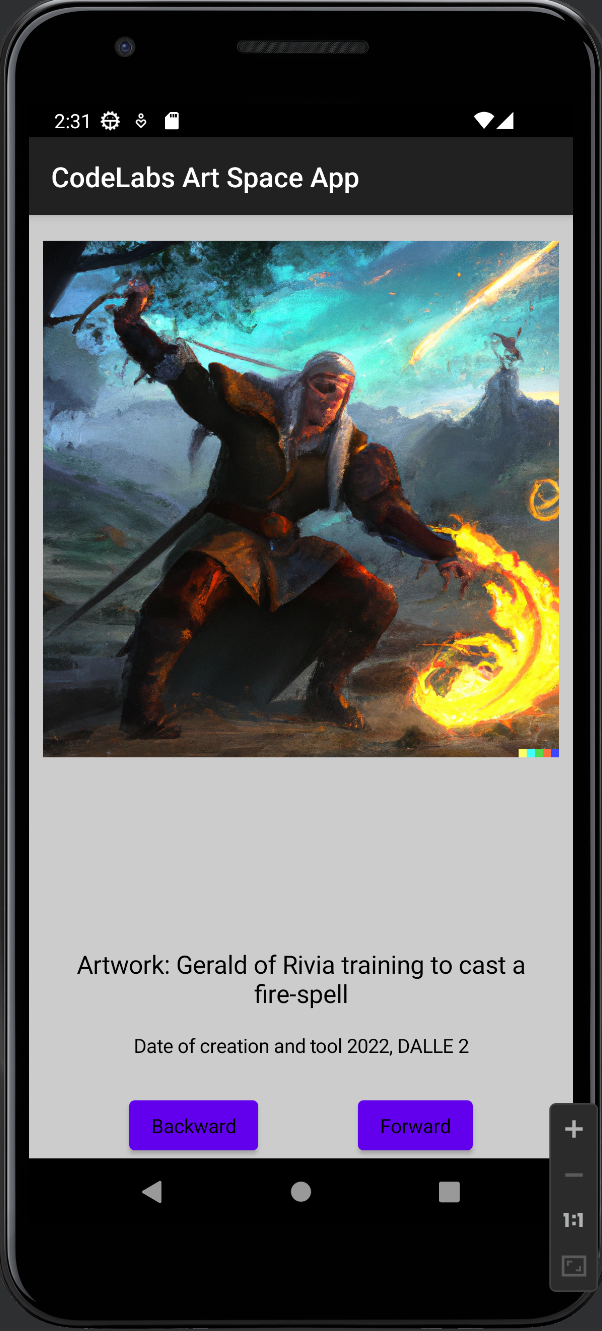
\includegraphics[width=.3\linewidth]{figures/app_screenshot_2.png}
	\caption{Screenshot of app screen in emulator of Android Studio}
	\label{fig:app_screen}
\end{figure}

\section{CodeLab: A report on usability}
% Basic examples :Hello World, Declare variables/functions, retaurn values --> beginner friendly, maybe a bit too easy for expirienced programmers?
% Advanced Tutorial: Graphical design similar to HTML, programming similar-ish to java o other high level languages

